\documentclass{article}


% if you need to pass options to natbib, use, e.g.:
%     \PassOptionsToPackage{numbers, compress}{natbib}
% before loading neurips_2022


% ready for submission
\usepackage[final]{neurips_2022}


% to compile a preprint version, e.g., for submission to arXiv, add add the
% [preprint] option:
%     \usepackage[preprint]{neurips_2022}


% to compile a camera-ready version, add the [final] option, e.g.:
%     \usepackage[final]{neurips_2022}


% to avoid loading the natbib package, add option nonatbib:
%    \usepackage[nonatbib]{neurips_2022}

\usepackage{amsmath}
\usepackage{graphicx}
\usepackage[utf8]{inputenc} % allow utf-8 input
\usepackage[T1]{fontenc}    % use 8-bit T1 fonts
\usepackage{hyperref}       % hyperlinks
\usepackage{url}            % simple URL typesetting
\usepackage{booktabs}       % professional-quality tables
\usepackage{amsfonts}       % blackboard math symbols
\usepackage{nicefrac}       % compact symbols for 1/2, etc.
\usepackage{microtype}      % microtypography
\usepackage{xcolor}         % colors


\title{A Survey on Distance Metric Learning}


% The \author macro works with any number of authors. There are two commands
% used to separate the names and addresses of multiple authors: \And and \AND.
%
% Using \And between authors leaves it to LaTeX to determine where to break the
% lines. Using \AND forces a line break at that point. So, if LaTeX puts 3 of 4
% authors names on the first line, and the last on the second line, try using
% \AND instead of \And before the third author name.


\author{%
  Litao Zhou \\
  Department of Computer Science\\
  University of Hong Kong\\
  \texttt{ltzhou@cs.hku.hk} \\
  % examples of more authors
  % \And
  % Coauthor \\
  % Affiliation \\
  % Address \\
  % \texttt{email} \\
  % \AND
  % Coauthor \\
  % Affiliation \\
  % Address \\
  % \texttt{email} \\
  % \And
  % Coauthor \\
  % Affiliation \\
  % Address \\
  % \texttt{email} \\
  % \And
  % Coauthor \\
  % Affiliation \\
  % Address \\
  % \texttt{email} \\
}



\begin{document}


\maketitle


\begin{abstract}
  In machine learning, there are many methods that require measuring the distance between data points. Traditionally, this is done by choosing some standard distance metric, such as Euclidean distance, and then applying it to the data. However, in many cases, the standard distance metric is not suitable for the data. In this paper, we survey the recent advances in distance metric learning, which aims to learn a distance metric that is suitable for the data.
  We will study various distance metric methods and compare them by training a KNN classifier based on each distance metric. The methods studied in this survey can be classified into three categories: traditional methods, supervised metric learning methods, and weakly-supervised metric learning methods. The advantages and disadvantages of each method are discussed at the end of the survey.
\end{abstract}

\section{Introduction}




In many machine learning tasks, it is important to select an appropriate distance measure for learning algorithms such as nearest neighbor searches, k-means clustering and so on. 
In this paper, we survey the recent advances in distance metric learning, which aims to learn a distance metric that is suitable for the data. We will study various distance metric methods and compare them by training a KNN classifier based on each distance metric. The methods studied in this survey can be classified into three categories: traditional methods, supervised metric learning methods, and weakly-supervised metric learning methods. 

The goal of distance measure is to measure the similarity/dissimilarity between two data points. Formally, given two data points $x$ and $y$, the goal of distance measure is to find a function $d$ computes a value $d(x,y)$ to characterize the distance between $x$ and $y$. \emph{Traditional methods} define this function $d$ as a fixed function, such as Euclidean distance, and then apply it to the data. However, in many cases, the standard distance metric is not suitable for the data, as each dimension of the data may have different importance. In this case, it is necessary to learn a distance metric that is suitable for the data. In other words, the distance function should be learned from the data, the process of which is called \emph{distance metric learning}.
Based on the way data points are used, distance metric learning can be classified into two categories: \emph{supervised metric learning} and \emph{weakly-supervised metric learning}. In supervised metric learning, the data points are paired with labels, and the goal is to learn a distance metric that separate the data points with different labels as far as possible. In weakly-supervised metric learning, the data points are not paired with labels, what is known is a set of constraints that certain pair/group of data points should be close/far to each other. The goal is to learn a distance metric that satisfies the constraints.

In this paper, we survey the recent advances in distance metric learning, which aims to learn a distance metric that is suitable for the data. We will study various distance metric methods and compare them by training a KNN classifier based on each distance metric. For every method, we will introduce the basic idea, demonstrate our experiment results and explain our analysis in this report. Most of our metric learning experiments adopt the implementations in \texttt{metric\_learn}\cite{metric-learn} library. 
The implementations can be found at \url{https://www.github.com/ltzhou0068/COMP9501}.

The rest of the survey is organized as follows. In Section \ref{sec:related}, we review the related works. In Section \ref{sec:method}, we introduce the setting of our experiments and the dataset used. In Section \ref{sec:experiment}, we present the experimental results. 
The advantages and disadvantages of each method are discussed in Section \ref{sec:conclusion} at the end of the survey.







\section{Related Works}
\label{sec:related}



\subsection{Traditional Distance Metrics}


\label{simple}

\subsubsection{Minkowski Distance}
The Minkowski distance of order $p$ (where $p$ is an integer) between two points $\mathbf{x}=\{x_1,x_2,\dots,x_n\}$ and $\mathbf{y}=\{y_1,y_2,\dots,y_n\}$ is defined as
$$d(\mathbf{x},\mathbf{y})=\left( \sum_{i=1}^n |x_i-y_i|^p\right)^{\frac{1}{p}}$$
When order $p$ in Minkowski distance varies, we can get different distance metrics.

\paragraph{Manhattan Distance}
When $p$ equals 1, we get Manhattan distance as
$$d(\mathbf{x},\mathbf{y})=\sum_{i=1}^n |x_i-y_i|$$

\paragraph{Euclidean Distance}
When $p$ equals 2, we have Euclidean distance as
$$d(\mathbf{x},\mathbf{y})=\sqrt{\sum_{i=1}^n (x_i-y_i)^2}$$
Euclidean distance is the most commonly used distance metric and it is the default metric in KNN of \texttt{sklearn}.

\paragraph{Chebyshev Distance}
In the limiting case of $p$ reaching infinity, we obtain the Chebyshev distance:
$$d(\mathbf{x},\mathbf{y})=\max_i |x_i-y_i|$$

\subsubsection{Cosine Distance}
Cosine similarity measures the similarity between two vectors of an inner product space. It is measured by the cosine of the angle between two vectors and determines whether two vectors are pointing in roughly the same direction.
$$\cos(\mathbf{x},\mathbf{y})=\frac{\mathbf{x}^T\mathbf{y}}{\|\mathbf{x}\|\|\mathbf{y}\|}$$

The resulting similarity ranges from $-1$ meaning exactly opposite, to 1 meaning exactly the same, with 0 indicating orthogonality or decorrelation. Therefore, the cosine distance is defined as,
$$d(\mathbf{x},\mathbf{y})=1-\cos(\mathbf{x},\mathbf{y})$$

When $\mathbf{x}$ and $\mathbf{y}$ are normalized to unit length, $\|\mathbf{x}\|=\|\mathbf{y}\|=1$, the relationship between Euclidean distance and cosine similarity is
$$d_{euc}(\mathbf{x},\mathbf{y})=\sqrt{2-2\cos(\mathbf{x},\mathbf{y})}$$



\subsection{Supervised Metric Learning}
% http://contrib.scikit-learn.org/metric-learn/supervised.html
\label{supervised}
    As the name suggests, Supervised Metric Learning takes each point x and its label y as an input, then it trys to learn a distance to make the samples in the same class have a relatively close measure while the samples in different classes have a far away distance with others. We show an intuitive example of metric learning in Figure \ref{fig:ml}. Commonly we project samples into the learned metric space and use several neighbors of samples as distance measure. Besides, sometimes the sample features are first reduced in dimension. In this section, we will use four supervised metric learning methods: LMNN, NCA, LFDA and MLKR.
    
    \begin{figure}[htbp]
        \centering
        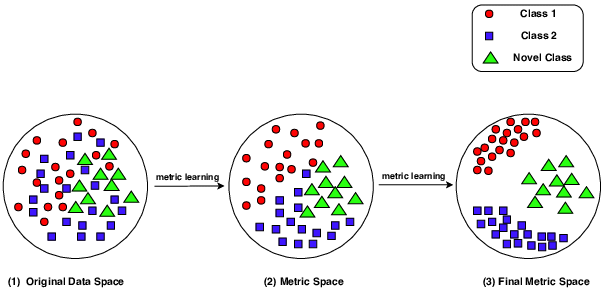
\includegraphics[width=0.7\linewidth]{img/metric-learning.png}
        \caption{An Intuitive Example of Metric Learning}
        \label{fig:ml}
    \end{figure}

\subsubsection{LMNN: Large Margin Nearest Neighbor Metric Learning}

    Large Margin Nearest Neighbor(LMNN)\cite{LMNN} classification is a supervised metric learning method based on sem-idefinite programming. This algorithm can be regarded as an optimization of KNN algorithm using Mahalanobis distance to some extent. 
    
    % As is well known, KNN takes some samples that has been classified in advance, then it calculates the distance between test sample and all trainning samples to select the k nearest samples to vote.
    As is well known, KNN usually takes simple distance metrics as its distance measure such as euclidean distance, manhattan distance. However, this makes all features weighted equally. To improve on that, LMNN tries to learn a Mahalanobis distance metric in the KNN classification setting.
    
     Suppose we have a distance metric methods:
     $$
        D_{\mathbf{L}}(x_i, x_j) = \|\mathbf{L}(x_i, x_j)\|_2^2
     $$
    when $\mathbf{M} = \mathbf{L}^T \mathbf{L}$, the Mahalanobis distance is defined as follow:
    $$
        D_{\mathbf{M}}(x_i, x_j) = (x_i - x_j)^T \mathbf{M} (x_i - x_j)
    $$
    Then the goal of distance measurement learning can be expressed in two aspects:
    (1) learn a linear transformation: $ \vec{x}' = \mathbf{L} \vec{x}$ (2) learn $\mathbf{M} = \mathbf{L}^T \mathbf{L}$. It is possible for some types of distance measures to learn convex optimizations on a cone represented by a positive semi-definite matrix $\mathbf{M}$.
    
    For LMNN, there are two aspects we should focus on: (1) Each training input $\vec{x}_i$ should have the same label $y_i$ as its k nearest neighbor samples. (2) If sample $\vec{x}_i$ and $\vec{x}_j$ with different labels should be widely separated during training.
    We define two loss function: $\varepsilon_{\text{pull}}$ corresponds to samples with same labels while $\varepsilon_{\text{push}}$ corresponds to the opposite:
    $$
    \begin{aligned}
       \varepsilon_{\text {pull }}(\mathbf{L}) &= \sum_{j \rightsquigarrow i}\left\|\mathbf{L}\left(\vec{x}_{i}-\vec{x}_{j}\right)\right\|^{2} \\
       \varepsilon_{\text {push }}(\mathbf{L}) &= \sum_{i, j \rightsquigarrow i} \sum_{l}\left(1-y_{i l}\right)\left[1+\left\|\mathbf{L}\left(\vec{x}_{i}-\vec{x}_{j}\right)\right\|^{2}-\left\|\mathbf{L}\left(\vec{x}_{i}-\vec{x}_{l}\right)\right\|^{2}\right]_{+}
    \end{aligned}
    $$
    merge two loss function, we get:
    $$
        \varepsilon(\mathbf{L}) = (1-\mu) \varepsilon_{\text {pull }}(\mathbf{L})+\mu \varepsilon_{\text {push }}(\mathbf{L})
    $$
    
    So the Object function is:
    $$
        \min \sum_{i, j} \mu_{ij} \| \mathbf{L}(\vec{x}_i - \vec{x}_j) \|^2 + c \sum_{i,j,l} \mu_{ij}(1 - y_{ij})\left [ 1 + \| \mathbf{L}(\vec{x}_i - \vec{x}_j) \|^2 - \| \mathbf{L}(\vec{x}_i - \vec{x}_l) \|^2 \right]_{+}
    $$
    An example of LMNN algorithm is shown in Figure \ref{fig:lmnn}:
    \begin{figure}[htbp]
        \centering
        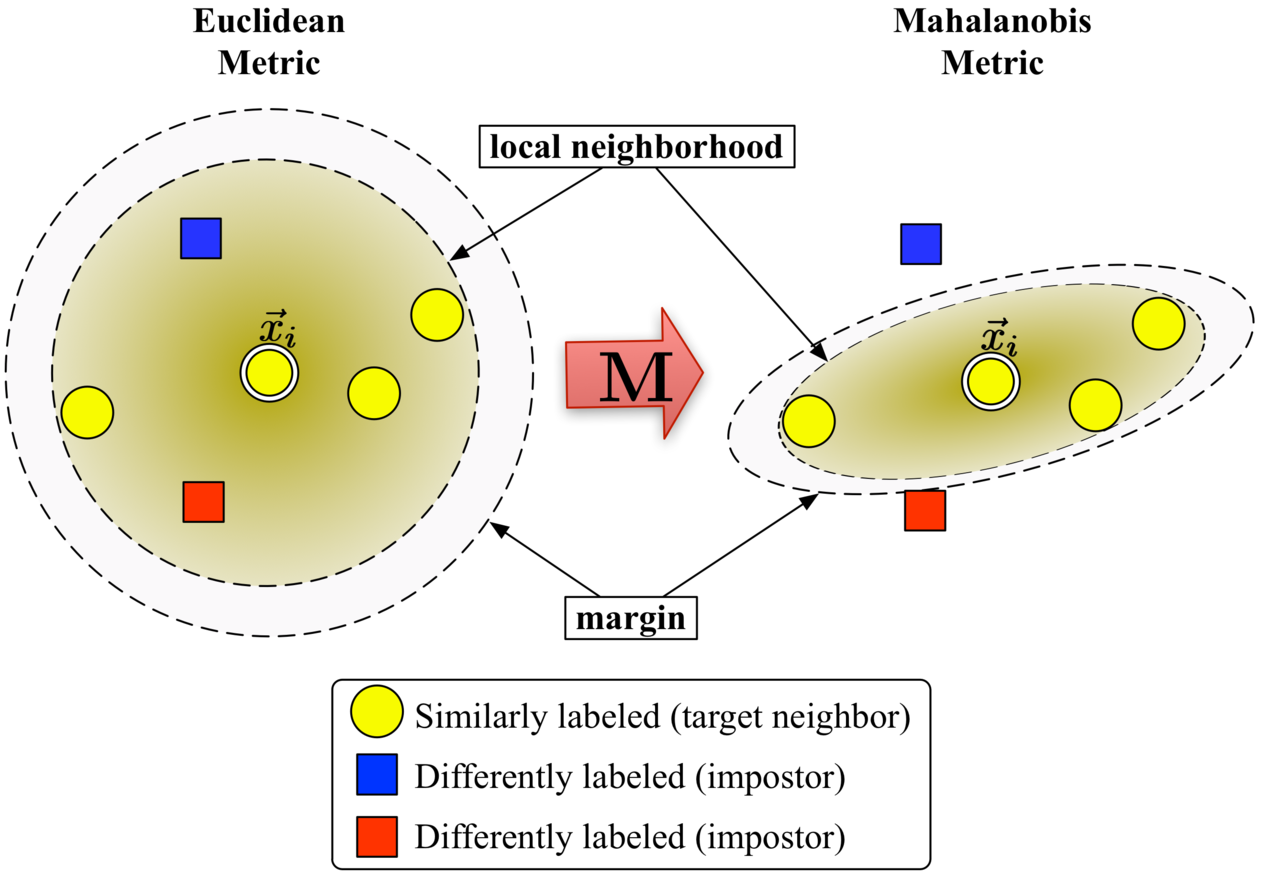
\includegraphics[width=0.6\linewidth]{img/Lmnn-principle.png}
        \caption{An Intuitive Example of LMNN Algorithm}
        \label{fig:lmnn}
    \end{figure}
    

        
\subsubsection{NCA: Neighborhood Components Analysis}


        Neighbourhood components analysis(NCA)\cite{NCA} algorithm is another supervised metric learning algorithm. The goal of NCA is similar as LMNN, it aims to classify input samples in different classes according to a learning metric distance. It find a linear transform of input samples to maximize the leave-one-out(LOO) classification performance.
        
        We have showed that the  Mahalanobis distance can be defined as: $D_{\mathbf{M}}(x_i, x_j) = (x_i - x_j)^T \mathbf{M} (x_i - x_j)$, where $\mathbf{M}$ is a  positive semi-definite matrix and can be expressed as $\mathbf{M} = \mathbf{L}^T \mathbf{L}$. We define an objective function $f(\cdot)$ to describe classification accuracy in the transformed space. Then the objective function:
        $$
            \mathbf{L}^* = \arg \max_{\mathbf{L}} f(\mathbf{L})
        $$
        The we need to make $f(\cdot)$ to be differential, so we define:
        $$
            f(\mathbf{L}) = \sum_i \sum_{j \in C_i} p_{ij} = \sum_i p_i
        $$
        where
        $$
            p_{i j}=\left\{
            \begin{array}{ll} 
                \frac{e^{-\left\|\mathbf{L} x_{i} - \mathbf{L} x_{j}\right\|^{2}}}{\sum_{k} e^{-\left\|\mathbf{L} x_{i}-\mathbf{L} x_{k}\right\|^{2}}}, & \text {if} \quad j \neq i \\
                0, & \text {if} \quad j=i
            \end{array}\right.
        $$
        $p_{ij}$ is the probability of classifying neighbor j of point i, $C_i$ is a data points set with same class as i. Then $f(\mathbf{L})$ can be differential to find the optimal solution.
        % \begin{aligned}
        %         \frac{e^{-\| Ax_i - Ax_j\|^2}}{\sum_k e^{-\| Ax_i - Ax_k\|^2}} \text{if} j \neq i \\
        %         0   \text{if} j = i
        %         \end{aligned}
        % classifying sample data to different classses according to the given distance metric. 
    
        
\subsubsection{LFDA: Local Fisher Discriminant Analysis}
    
        Local Fisher Discriminant Analysis(LFDA)\cite{LFDA} algorithm is a combination of Linear Discriminant Analysis(LDA) and Locality-Preserving Projection(LPP), where LDA aims at maximize the distance of data between classes and minimize the distance within classes and LPP can keeps nearby data pairs also be closed in the embedding space. So LFDA has good performance in dealing with multi-modality for it preserves original data structure.
        
        LDFA defines matrix distances in pairs which is similar to LDA: the Fisher local scatter matrix within class is
        $$
            \mathbf{S}^{(w)} =\frac{1}{2} \sum_{i, j=1}^{n} W_{i j}^{(w)}\left(\mathbf{x}_{i}-\mathbf{x}_{j}\right)\left(\mathbf{x}_{i}-\mathbf{x}_{j}\right)^{T}
        $$
        and between class is:
        $$
            \mathbf{S}^{(b)} =\frac{1}{2} \sum_{i, j=1}^{n} W_{i j}^{(b)}\left(\mathbf{x}_{i}-\mathbf{x}_{j}\right)\left(\mathbf{x}_{i}-\mathbf{x}_{j}\right)^{T}
        $$
        where
        $$
            W_{i j}^{(w)}=\left\{
            \begin{array}{ll}
                0 \quad  & y_{i} \neq y_{j} \\
                \mathbf{A}_{i, j} / n_{l} \quad  & y_{i}=y_{j}
            \end{array}\right.
        $$
        $$
            W_{i j}^{(b)}=\left\{
            \begin{array}{ll}
                1 / n & y_{i} \neq y_{j} \\
                \mathbf{A}_{i, j}\left(1 / n-1 / n_{l}\right) & y_{i}=y_{j}
            \end{array}\right.
        $$
        $n$ denotes the total number of samples and $n_l$ denotes the number of samples in class $l$.
        
        The object function of LFDA is defined as:
        $$
            \mathbf{L}_{L F D A}=\arg \max _{\mathbf{L}}\left[\operatorname{tr}\left(\left(\mathbf{L}^{T} \mathbf{S}^{(w)} \mathbf{L}\right)^{-1} \mathbf{L}^{T} \mathbf{S}^{(b)} \mathbf{L}\right)\right]
        $$
        An example of LFDA algorithm is shown in Figure \ref{fig:lfda}:
        \begin{figure}[htbp]
            \centering
            \includegraphics[width=0.6\linewidth]{img/Lfda-principle.png}
            \caption{An Intuitive Example of LMNN Algorithm}
            \label{fig:lfda}
        \end{figure}
    

\subsubsection{MLKR: Metric Learning for Kernel Regression}
    
    
         Metric Learning for Kernel Regression(MLKR)\cite{MLKR} algorithm proposed a new strategy based on kernel regression, which can be applied with many types of kernel functions and distance metrics. It learns a distance function by minimizing the error of leave-one-out regression.
         
         The loss function is defined as
         $$
            \mathcal{L} = \sum_i (y_i - \hat{y_i})^2
         $$
         where $\hat{y_i}$ is a sample prediction get from kernel regression:
         $$
            \hat{y_i} = \frac{\sum_{j \neq i} y_i k_{ij}}{\sum_{j \neq i} k_{ij}}
         $$
         $k_{ij}$ is the weight defined as
         $$
            k_{ij} = \frac{1}{\sqrt{2 \pi} \sigma} \exp \left ( -\frac{d(\mathbf{x}_i, \mathbf{x}_j)}{\sigma^2}\right)
         $$
         where $d(\cdot, \cdot)$ is Mahalanobis distance. $d(\mathbf{x}_i, \mathbf{x}_j) = \| \mathbf{L} (\mathbf{x}_i - \mathbf{x}_j)  \|$.



\subsection{Weakly Supervised Metric Learning}

\label{weaksupervised}
There are also a group of metric learning methods based on pairs or triples of similar and dissimilar points. Since they pose fewer demands on the training data-set, we will refer to them as \emph{Weakly Supervised Metric Learning} methods. In this paper, we study four weakly supervised metric learning methods, namely ITML, LSML, SCML and RCA.




\subsubsection{ITML: Information Theoretic Metric Learning}

ITML\cite{ITML} minimizes the (differential) relative entropy (Kullback-Leibler divergence), between two multivariate Gaussians subject to constraints on the associated Mahalanobis distance, which can be formulated into a Bregman optimization problem by minimizing the LogDet divergence subject to linear constraints. This algorithm can handle a wide variety of constraints and can optionally incorporate a prior on the distance function. Unlike some other methods, ITML does not rely on an eigenvalue computation or semi-definite programming.

Given a Mahalanobis distance parameterized by $M$, its corresponding multivariate Gaussian is denoted as:
$$
p(\mathbf{x} ; \mathbf{M})=\frac{1}{Z} \exp \left(-\frac{1}{2} d_{\mathbf{M}}(\mathbf{x}, \mu)\right)=\frac{1}{Z} \exp \left(-\frac{1}{2}\left((\mathbf{x}-\mu)^{T} \mathbf{M}(\mathbf{x}-\mu)\right)\right)
$$
where $Z$ is the normalization constant, the inverse of Mahalanobis matrix $\mathbf{M}^{-1}$ is the covariance of
the Gaussian.


The ITML method is based on truth of similar/dissimilar pairs, which we will sample from the labeled groups. Given pairs of similar points $S$ and pairs of dissimilar points $D$, the distance metric learning problem is to minimize the LogDet divergence, which is equivalent as minimizing $\mathbf{K} \mathbf{L}\left(p\left(\mathbf{x} ; \mathbf{M}_{0}\right) \| p(\mathbf{x} ; \mathbf{M})\right)$
$$
\begin{array}{rl}
\min _{\mathbf{A}} D_{\ell \mathrm{d}}\left(M, M_{0}\right)& =\operatorname{tr}(\left.M M_{0}^{-1}\right)-\log \operatorname{det}\left(M M_{0}^{-1}\right)-n \\
\text { subject to } &d_{\mathbf{M}}\left(\mathbf{x}_{i}, \mathbf{x}_{j}\right) \leq u \quad \left(\mathbf{x}_{i}, \mathbf{x}_{j}\right) \in S \\
& d_{\mathbf{M}}\left(\mathbf{x}_{i}, \mathbf{x}_{j}\right) \geq l \quad \left(\mathbf{x}_{i}, \mathbf{x}_{j}\right) \in D
\end{array}
$$
where $u$ and $l$ is the upper and the lower bound of distance for similar and dissimilar pairs respectively, and $\mathbf{M}_{0}$ is the prior distance metric, set to identity matrix by default, $D_{\ell \mathrm{d}}(\cdot, \cdot)$ is the log determinant.

 
\subsubsection{LSML: Least Squared-residual Metric Learning}

LSML\cite{LSML} proposes a loss function for metric learning based on the relative distance comparison results of pairs. The loss function of each constraint $d\left(\mathbf{x}_{i}, \mathbf{x}_{j}\right)<d\left(\mathbf{x}_{k}, \mathbf{x}_{l}\right)$ is denoted as:
$$
\boldsymbol{H}\left(d_{\mathbf{M}}\left(\mathbf{x}_{i}, \mathbf{x}_{j}\right)-d_{\mathbf{M}}\left(\mathbf{x}_{k}, \mathbf{x}_{l}\right)\right)
$$
where $H(\cdot)$ is the squared Hinge loss function defined as:
$$
H(x)=\left\{\begin{array}{ll}
0 & x \leq 0 \\
x^{2} & x>0
\end{array}\right.
$$
The summed loss function $L(C)$ is the simple sum over all constraints $\boldsymbol{C}=\left\{\left(\mathbf{x}_{i}, \mathbf{x}_{j}, \mathbf{x}_{k}, \mathbf{x}_{l}\right): d\left(\mathbf{x}_{i}, \mathbf{x}_{j}\right)<d\left(\mathbf{x}_{k}, \mathbf{x}_{l}\right)\right\} .$ 

The distance metric learning problem becomes minimizing the summed loss function of all constraints plus a regularization term w.r.t. the prior knowledge:

$$
\min _{\mathbf{M}}\left(D_{l d}\left(\mathbf{M}, \mathbf{M}_{\mathbf{0}}\right)+\sum_{\left(\mathbf{x}_{i}, \mathbf{x}_{j}, \mathbf{x}_{k}, \mathbf{x}_{l}\right) \in C} H\left(d_{\mathbf{M}}\left(\mathbf{x}_{i}, \mathbf{x}_{j}\right)-d_{\mathbf{M}}\left(\mathbf{x}_{k}, \mathbf{x}_{l}\right)\right)\right)
$$

where $\mathbf{M}_{0}$ is the prior metric matrix, set as identity by default, $D_{l d}(\cdot, \cdot)$ is the LogDet divergence:

$$
\boldsymbol{D}_{l d}\left(\mathbf{M}, \mathbf{M}_{\mathbf{0}}\right)=\operatorname{tr}\left(\mathbf{M M}_{\mathbf{0}}\right)-\log \operatorname{let}(\mathbf{M})
$$

The minimizing goal is a convex objective function corresponding to the sum of squared residuals of constraints. The algorithm is considered as a simple, yet effective, algorithm since its sparsity extension leads to more stable estimation when the dimension is high and only a small amount of constraints is given.








\subsubsection{SCML: Sparse Compositional Metric Learning}

Some weakly supervised metric learning are based on \emph{triplet} samples. The semantic of a triplet of data-point is that the first point should be closer to the second point than to the third one.

SCML\cite{SCML} learns a squared Mahalanobis distance from triplet constraints by optimizing sparse positive weights assigned to a set of $K$ rank-one PSD bases. This can be formulated as an optimization problem with only $K$ parameters, that can be solved with an efficient stochastic composite scheme.
The Mahalanobis matrix $M$ is built from a basis set $B=\left\{b_{i}\right\}_{i=\{1, \ldots, K\}}$ weighted by a $K$ dimensional vector $w=\left\{w_{i}\right\}_{i=\{1, \ldots, K\}}$ as:
$$
M=\sum_{i=1}^{K} w_{i} b_{i} b_{i}^{T}=B \cdot \operatorname{diag}(w) \cdot B^{T} \quad w_{i} \geq 0
$$
Learning $M$ in this form makes it PSD by design, as it is a nonnegative sum of PSD matrices. The basis set $B$ is fixed in advance and it is possible to construct it from the data. The optimization problem over $w$ is formulated as a classic margin-based hinge loss function involving the set $C$ of triplets. A regularization $\ell_{1}$ is added to yield a sparse combination. The formulation is the following:
$$
\min _{w \geq 0} \sum_{\left(x_{i}, x_{j}, x_{k}\right) \in C}\left[1+d_{w}\left(x_{i}, x_{j}\right)-d_{w}\left(x_{i}, x_{k}\right)\right]_{+}+\beta\|w\|_{1}
$$
where $[\cdot]_{+}$ is the hinge loss.




\subsubsection{RCA: Relative Components Analysis}

RCA\cite{RCA1,RCA2,RCA3} learns metrics by pairs. It will generate a full rank Mahalanobis distance metric based on a weighted sum of \emph{in-chunklets} covariance matrices. It applies a global linear transformation to assign large weights to relevant
dimensions and low weights to irrelevant dimensions. Those relevant dimensions are estimated using \emph{``chunklets''}, subsets of points that are known to belong to the same class.

We will sample \texttt{chunk\_size} training points for each \texttt{num\_chunks} chunklets, so that the algorithm is efficient by simply computing
$$
\mathbf{C}=\frac{1}{n} \sum_{j=1}^{k} \sum_{i=1}^{n_{j}}\left(\mathbf{x}_{j i}-\hat{\mathbf{m}}_{j}\right)\left(\mathbf{x}_{j i}-\hat{\mathbf{m}}_{j}\right)^{T}
$$
where chunklet $j$ consists of $\left\{\mathbf{x}_{j i}\right\}_{i=1}^{n_{j}}$ with a mean $\hat{m}_{j} .$ The inverse of $\mathbf{C}^{-1}$ is used as the Mahalanobis matrix.



\section{Methodology}
\label{sec:method}


\subsection{Dataset}

Animals with Attributes (AwA2) data-set\footnote{\texttt{https://cvml.ist.ac.at/AwA2/}}~\cite{xian2018zero} consists of 37322 images of 50 animal classes with pre-extracted deep learning features for each image. We will use this data-set to explore different distance metrics. Throughout this project, we will be using KNN (implemented in \texttt{sklearn.neighbors.KNeighborsClassifier}) to perform classification tasks on the data-set.

\begin{table}[htbp]
\centering
\caption{Cross Validation Accuracy of KNN on Raw Data under Different Settings of $K$ }
\label{tab:cross-val}
\begin{tabular}{@{}ccccccc@{}}
\toprule
$K$    & Fold 1  & Fold 2  & Fold 3  & Fold 4  & Fold 5  & Avg Accuracy \\ \midrule
1   & 87.83\% & 87.27\% & 88.26\% & 87.87\% & 88.25\% & 87.90\%      \\
2   & 86.31\% & 85.38\% & 86.74\% & 86.00\% & 86.20\% & 86.13\%      \\
3   & 88.75\% & 87.81\% & 88.84\% & 87.78\% & 88.41\% & 88.32\%      \\
4   & 88.79\% & 87.83\% & 89.37\% & 88.23\% & 88.43\% & 88.53\%      \\
5   & 89.15\% & 88.43\% & 89.86\% & 88.72\% & 88.92\% & 89.02\%      \\
6   & 88.99\% & 88.35\% & 89.64\% & 88.88\% & 88.83\% & 88.94\%      \\
7   & 89.04\% & 88.79\% & 89.91\% & 88.77\% & 88.74\% & \textbf{89.05\%}      \\
8   & 89.04\% & 88.59\% & 89.82\% & 88.34\% & 88.37\% & 88.83\%      \\
9   & 88.99\% & 88.50\% & 89.57\% & 88.63\% & 88.57\% & 88.85\%      \\
10   & 88.84\% & 88.32\% & 89.33\% & 88.52\% & 88.37\% & 88.68\%      \\\bottomrule
\end{tabular}
\end{table}

To ensure the consistency in different experiments, we split the images in each category into 60\% for training and 40\% for testing. Throughout all experiments, the same training set will be used and accuracy results will be obtained from the testing set.

To begin with, we use K-fold cross-validation within the training set to determine the hyper-parameter $K$ for KNN model. The training set is split into 5 folds and the distance used is Euclidean distance. The cross-validation results of $K$ ranging from 1 to 10 are displayed in Table \ref{tab:cross-val}. We visualize the average score of $K$ ranging from 1 to 30 in Figure \ref{fig:cvk}. We can get optimal accuracy when $K$ equals 7, and when $K$ goes larger than 7, the accuracy shows a downward trend.

\begin{figure}
    \centering
    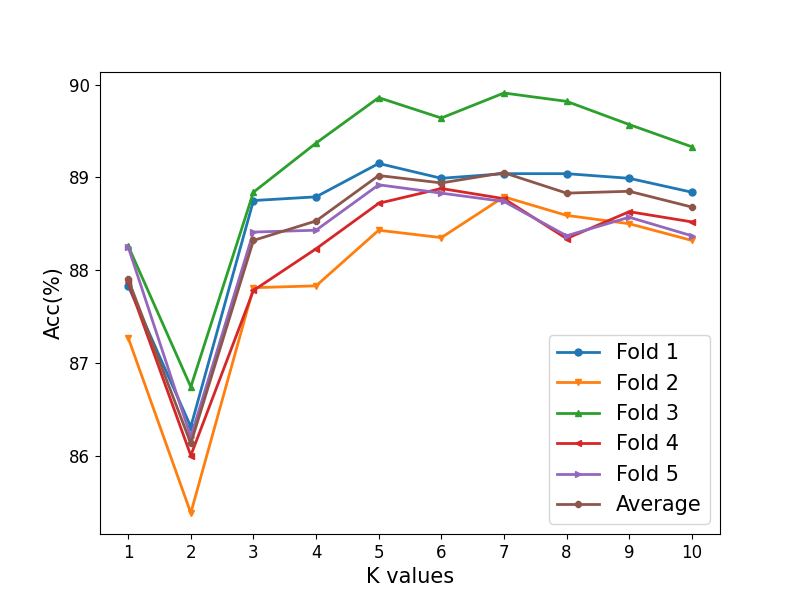
\includegraphics[width=0.6\textwidth]{img/KNN_res.png}
    \caption{Cross Validation Accuracy over $K$}
    \label{fig:cvk}
\end{figure}


\subsection{Experiment setting}

As different distance metrics may get different optimal $K$ value, in the following experiments, we test on $K$ from 3 to 10, 15 and 20. For traditional metrics, the distance is calculated directly. For supervised metric learning methods, we make use of the original labels to train the distance metric. 

For weakly-supervised metric learning methods, since they require pairs/groups of similar/dissimilar data points,
we will sample similar and dissimilar points from the labeled data-set. To be specific, for pairs learners, pairs (tuple of two points from the data-set), and pair labels (integer indicating whether the two points are similar (+1) or dissimilar (-1)), are sampled randomly from the original data-set with category labels. To sample positive pairs (of label +1), the method will look at all the samples from the same label and sample randomly a pair among them. To sample negative pairs (of label -1), the method will look at all the samples from a different class and sample randomly a pair among them.


\section{Experiments}
\label{sec:experiment}


\subsection{Traditional Distance Metrics}

The testing results of the simple distance metrics above are shown in Table \ref{tab:simple}. We can see that among three Minkowski distances, Euclidean distance gets an accuracy one percent higher than Manhattan. However, Chebyshev distance perfroms much worse than them for a gap around 10\%. Cosine distance also performs well for an accuracy above 90\%, and we also note that the classifier using Cosine distance 
computes fastest in these metrics.

\begin{table}[htbp]
    \centering
    \caption{Accuracy of KNN with Simple Distance Metrics}
    \begin{tabular}{@{}ccccc@{}}
    \toprule
    $K$     &   Manhattan   &   Euclidean   &   Chebyshev   &   Cosine  \\ \midrule
    3       &   88.18\%     &   88.83\%     &   77.69\%     &  89.85\%  \\
    4       &   88.04\%     &   88.89\%     &   78.30\%     &   89.80\% \\
    5       &   \textbf{88.50\%} &   89.27\%&   78.61\%     &   90.37\% \\
    6       &   88.33\%     &   89.33\%     &   78.81\%     &   90.13\% \\
    7       &   88.48\%     &   \textbf{89.45\%} &   \textbf{79.17\%}   &   \textbf{90.53\%}   \\ 
    8       &   88.09\%     &   89.10\%     &   78.83\%     &   90.43\% \\
    9       &   88.30\%     &   89.18\%     &   79.14\%     &   90.41\% \\
    10      &   88.06\%     &   89.16\%     &   78.91\%     &   90.44\% \\
    15      &   87.58\%     &   88.89\%     &   78.48\%     &   90.37\% \\
    20      &   87.05\%     &   88.68\%     &   78.03\%     &   90.17\% \\\bottomrule
    \end{tabular}
    \label{tab:simple}
\end{table}



\subsection{Supervised Metric Learning}


\subsubsection{LMNN: Large Margin Nearest Neighbor Metric Learning}
% todo
In this section, there are two "k" values which has a big influence on experiment result. The first one matters in LMNN metric learning process, denoted as $K_1$,  and the other one is used in KNN classifying process, denoted as $K_2$. we take different $K_1$ and $K_2$ on this experiment and get the result in table \ref{tab:lmnn_k}.
\begin{table}[htbp]
\centering
\caption{KNN Accuracy of LMNN with K neighbors}
\scriptsize
\begin{tabular}{@{}cccccccccccc@{}}
\toprule
$K_1 \backslash K_2$ & 3 & 4 & 5 & 6 & 7 & 8 & 9 & 10 & 15 & 20 \\ \midrule
3 & 90.77\% & 91.04\% & 91.41\% & 91.44\% & 91.51\% & 91.42\% & 91.75\% & 91.69\% & 91.60\% & 91.28\% \\
7 & 91.84\% & 91.98\% & 92.18\% & 92.36\% & 92.44\% & 92.26\% & 92.37\% & 92.40\% & 92.18\% & 92.15\% \\
10 & 91.83\% & 92.12\% & 92.26\% & 92.36\% & 92.58\% & 92.58\% & 92.63\% & 92.54\% & 92.52\% & 92.42\% \\
15 & 92.20\% & 92.39\% & 92.68\% & 92.48\% & 92.58\% & 92.63\% & 92.74\% & 92.71\% & 92.71\% & 92.62\% \\
20 & 92.52\% & 92.32\% & 92.73\% & 92.62\% & 92.89\% & 92.68\% & 92.85\% & 92.79\% & 92.80\% & 92.79\% \\
30 & 90.38\% & 90.75\% & 91.39\% & 91.23\% & 91.55\% & 91.56\% & 91.58\% & 91.65\% & 91.75\% & 91.83\% \\
\bottomrule
\end{tabular}
\label{tab:lmnn_k}
\end{table}

We can the accuracy trend in fig\ref{fig:lmnn_k}. As is shown, when $K_1$ takes the value 20, KNN has a relatively good classification performance as a whole. This is related to the distribution of samples. When K1 is too small, it is not enough to learn a suitable projection with the help of neighbors; While when K1 is too large, it is easy to introduce disturbing neighbor samples.
\begin{figure}
\centering
\begin{minipage}[t]{0.48\linewidth}
\centering
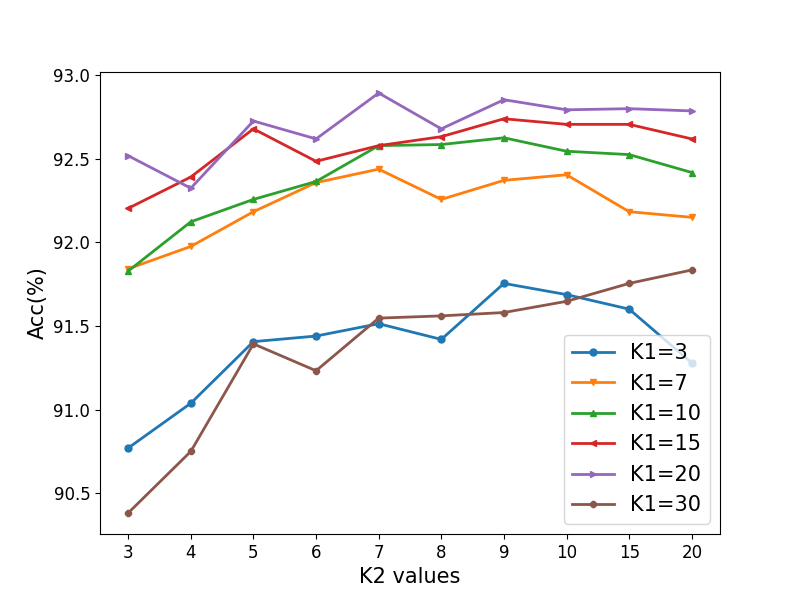
\includegraphics[width=1.0\linewidth]{img/LMNN_K.png}
\caption{The Influence of K values on Result}
\label{fig:lmnn_k}
\end{minipage}
\begin{minipage}[t]{0.48\linewidth}
\centering
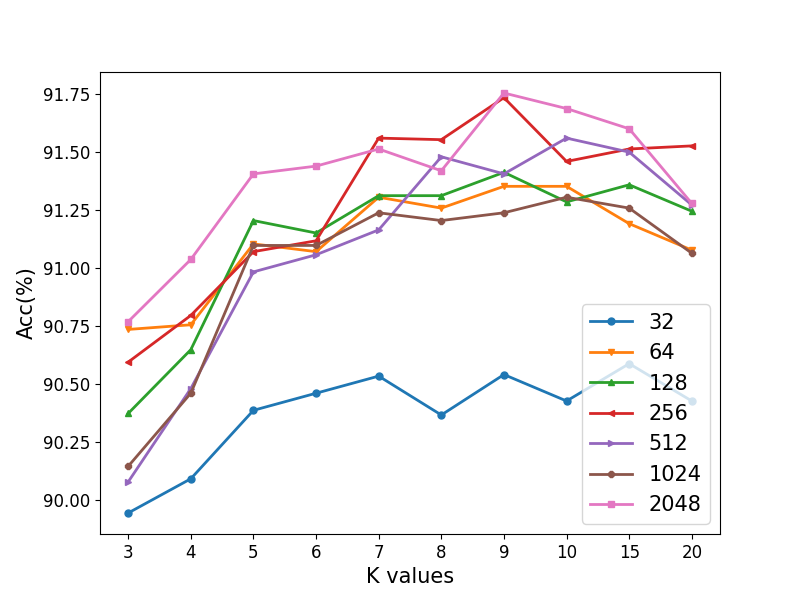
\includegraphics[width=1.0\linewidth]{img/LMNN_res.png}
\caption{The Influence of Feature Dimensions on Result}
\label{fig:lmnn_res}
\end{minipage}
\end{figure}


We also selected different degrees of dimensionality reduction to observe the influence of feature dimensions on the final classification. We show the result and trend in table \ref{tab:lmnn} and fig \ref{fig:lmnn_res}. For LMNN algorithm, The best classification effect is achieved by retaining the original features. However, with the increase of K parameter in KNN, it shows a downward trend. In general, when K is small, it is better to keep the higher dimension, and when K is large, reducing the dimension to 256 achieves a better result.


\begin{table}[htbp]
\centering
\caption{KNN Accuracy of LMNN with Different Features}
\begin{tabular}{@{}cccccccc@{}}
\toprule
$K_2 \backslash $Features & 32 & 64 & 128 & 256 & 512 & 1024 & 2048 \\ \midrule
3 & 89.946\% & 90.736\% & 90.374\% & 90.595\% & 90.080\% & 90.147\% & 90.770\% \\
4 & 90.093\% & 90.756\% & 90.649\% & 90.796\% & 90.482\% & 90.462\% & 91.038\% \\
5 & 90.388\% & 91.105\% & 91.205\% & 91.071\% & 90.984\% & 91.098\% & 91.406\% \\
6 & 90.462\% & 91.071\% & 91.151\% & 91.118\% & 91.058\% & 91.098\% & 91.439\% \\
7 & 90.535\% & 91.306\% & 91.312\% & 91.560\% & 91.165\% & 91.239\% & 91.513\% \\
8 & 90.368\% & 91.259\% & 91.312\% & 91.553\% & 91.480\% & 91.205\% & 91.419\% \\
9 & 90.542\% & \textbf{91.352\%} & \textbf{91.413\%} & \textbf{91.734\%} & 91.406\% & 91.239\% & \textbf{91.754\%} \\
10 & 90.428\% & 91.352\% & 91.285\% & 91.460\% & \textbf{91.560\%} & \textbf{91.306\%} & 91.687\% \\
15 & \textbf{90.589\%} & 91.192\% & 91.359\% & 91.513\% & 91.500\% & 91.259\% & 91.6\% \\
20 & 90.428\% & 91.078\% & 91.245\% & 91.527\% & 91.272\% & 91.064\% & 91.279\% \\
\bottomrule
\end{tabular}
\label{tab:lmnn}
\end{table}


\subsubsection{NCA: Neighborhood Component Analysis}
        % to do
        For NCA algorithm, the two parameters that have influence on the result comparison are sample feature dimension and the number of neighbors in KNN cluster. We take different values on these two variables and get the result in table \ref{tab:nca}.
\begin{table}[htbp]
    \centering
    \caption{KNN Accuracy of NCA with Different Features}
    \begin{tabular}{@{}cccccccc@{}}
    \toprule
    $K \backslash $Features & 32 & 64 & 128 & 256 & 512 & 1024 & 2048 \\ \midrule
    3 & 90.019\% & 88.827\% & 88.841\% & 88.753\% & 88.566\% & 88.211\% & 87.943\% \\
    4 & 90.180\% & 88.854\% & 89.242\% & 88.887\% & 88.586\% & 88.191\% & 88.057\% \\
    5 & 90.622\% & 89.410\% & 89.611\% & 89.175\% & 88.995\% & 88.392\% & 88.432\% \\
    6 & 90.488\% & 89.229\% & 89.631\% & 89.336\% & 89.088\% & 88.512\% & 88.224\% \\
    7 & 90.703\% & 89.604\% & 89.671\% & \textbf{89.638\%} & \textbf{89.343\%} & \textbf{88.948\%} & 88.519\% \\
    8 & 90.716\% & 89.490\% & 89.731\% & 89.551\% & 89.169\% & 88.566\% & 88.385\% \\
    9 & 90.823\% & \textbf{89.658\%} & 89.651\% & 89.417\% & 89.276\% & 88.82\% & \textbf{88.546\%} \\
    10 & 90.723\% & 89.497\% & \textbf{89.792\%} & 89.396\% & 89.095\% & 88.606\% & 88.432\% \\
    15 & 90.850\% & 89.504\% & 89.671\% & 89.283\% & 88.834\% & 88.184\% & 88.110\% \\
    20 & \textbf{90.897\%} & 89.142\% & 89.363\% & 88.794\% & 88.432\% & 87.796\% & 87.675\% \\ \bottomrule
    \end{tabular}
    \label{tab:nca}
\end{table}

    We look at the results in a line chart \ref{fig:nca_res}. The K value for maximum accuracy varies with the selection of feature dimensions, but the overall range is between 7 and 10. This indicates that when a dimension that can fully distinguish features is maintained, a moderate range of K values can be selected to achieve better results. 
    
    In addition, the dimension reduction to 32-dimensional features in this experiment can achieve a surprising accuracy, which is confused. We believe that this simplified feature is more conducive to NCA learning better projection methods in the neighborhood.
    \begin{figure}[htbp]
        \centering
        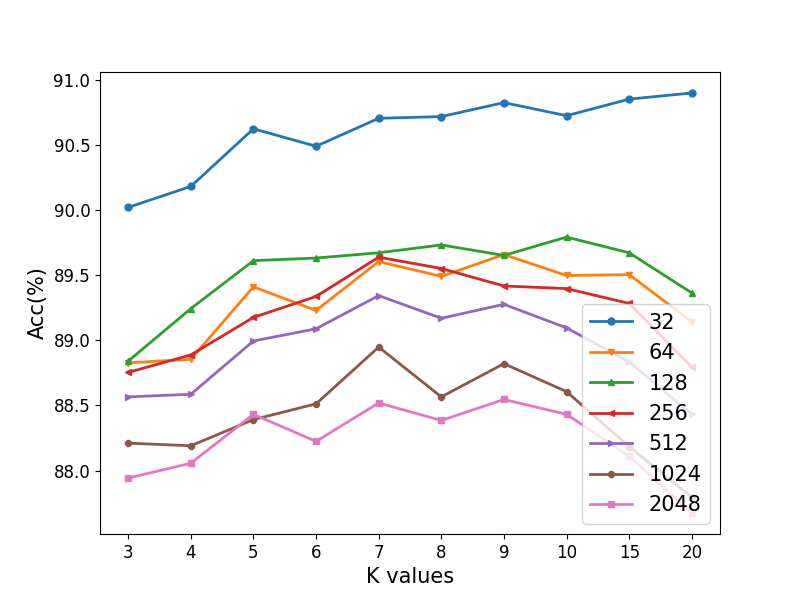
\includegraphics[width=0.6\linewidth]{img/NCA_res.png}
        \caption{The Result of NCA}
        \label{fig:nca_res}
    \end{figure}



\subsubsection{LFDA: Local Fisher Discriminant Analysis}
        Similar to LMNN method, $K_1$ and $K_2$ were selected here for the first experiment, and K2 and characteristic dimension, were selected for the second experiment. We show the result in table \ref{tab:lfda_k} and \ref{tab:lfda}.
        
        From the result we can see that when $K_1$ equals to 20, The performance is optimal overall. One thing to notice is that when $K_1$ takes 3 and 7, there is no any effect on the results. This has to do with the distribution of sample features, when we take different K value on a small scale, neighbors of the sample did not change the LFDA results. And there is also a trend that when we increase $K_2$ in a range greater than 7, the overall performance of KNN classification shows decline.
        
         Another factor is feature dimension. We can find that when the number of features is a moderate value such as 64, 128, 256, KNN classification can achieve the best results which is different from LMNN methods.
        
\begin{table}[htbp]
    \centering
    \caption{KNN Accuracy of LFDA with K neighbors}
    \scriptsize
    \begin{tabular}{@{}cccccccccccc@{}}
    \toprule
    $K_1 \backslash K_2$ & 3 & 4 & 5 & 6 & 7 & 8 & 9 & 10 & 15 & 20 \\ \midrule
    3 & 86.33\% & 86.18\% & 86.68\% & 86.34\% & 86.5\% & 86.32\% & 86.3\% & 86.21\% & 85.92\% & 85.52\% \\
    7 & 86.33\% & 86.18\% & 86.68\% & 86.34\% & 86.5\% & 86.32\% & 86.3\% & 86.21\% & 85.92\% & 85.52\% \\
    10 & 86.04\% & 85.82\% & 86.05\% & 85.77\% & 86.01\% & 85.79\% & 85.81\% & 85.69\% & 85.52\% & 85.04\% \\
    15 & 86.17\% & 86.21\% & 86.53\% & 86.46\% & 86.37\% & 86.42\% & 86.44\% & 86.25\% & 86.09\% & 85.74\% \\
    20 & 86.96\% & 86.82\% & 87.01\% & 86.94\% & 86.94\% & 86.75\% & 86.87\% & 86.72\% & 86.56\% & 86.31\% \\
    30 & 85.51\% & 85.42\% & 85.61\% & 85.52\% & 85.59\% & 85.32\% & 85.48\% & 85.22\% & 85.1\% & 84.53\% \\
    \bottomrule
    \end{tabular}
    \label{tab:lfda_k}
\end{table}
    \begin{figure}
        \centering
        \begin{minipage}[t]{0.48\linewidth}
            \centering
            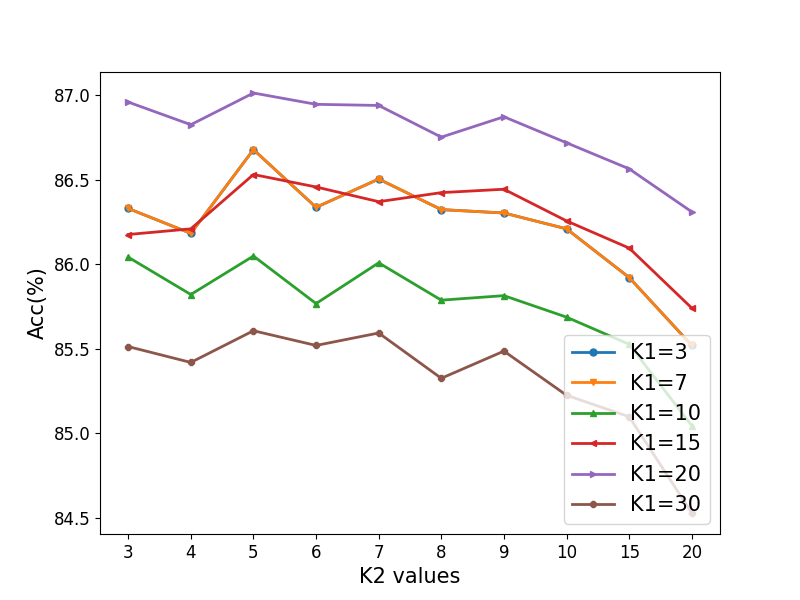
\includegraphics[width=1.0\linewidth]{img/LFDA_K.png}
            \caption{The Influence of K values on Result}
            \label{fig:lfda_k}
        \end{minipage}
        \begin{minipage}[t]{0.48\linewidth}
            \centering
            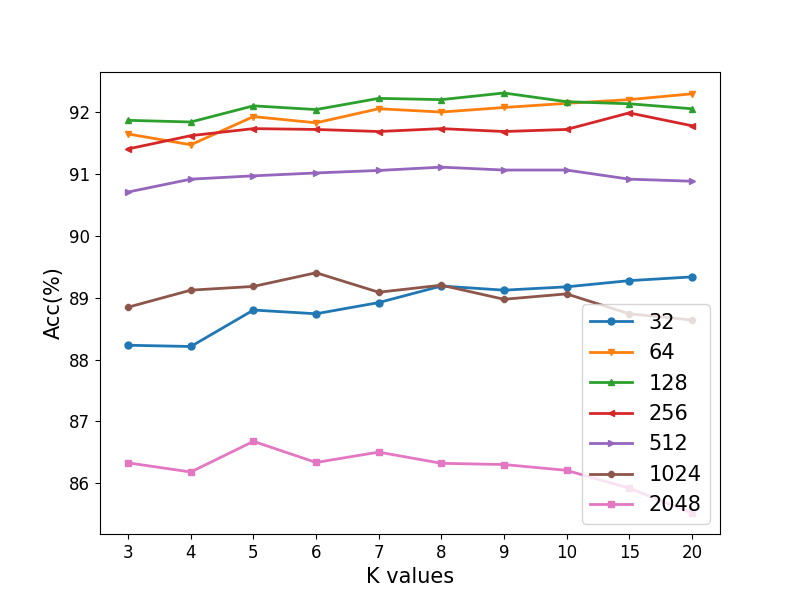
\includegraphics[width=1.0\linewidth]{img/LFDA_res.png}
            \caption{The Influence of Feature Dimensions on Result}
            \label{fig:lfda_res}
        \end{minipage}
    \end{figure}
    
\begin{table}[htbp]
    \centering
    \caption{KNN Accuracy of LFDA with Different Features}
    \begin{tabular}{@{}cccccccc@{}}
    \toprule
    $K_2 \backslash $Features & 32 & 64 & 128 & 256 & 512 & 1024 & 2048 \\ \midrule
    3 & 88.231\% & 91.647\% & 91.868\% & 91.406\% & 90.709\% & 88.847\% & 86.329\% \\
    4 & 88.211\% & 91.473\% & 91.841\% & 91.620\% & 90.917\% & 89.122\% & 86.181\% \\
    5 & 88.800\% & 91.928\% & 92.103\% & 91.734\% & 90.971\% & 89.182\% & \textbf{86.677\%} \\
    6 & 88.740\% & 91.828\% & 92.042\% & 91.721\% & 91.017\% & \textbf{89.403\%} & 86.335\% \\
    7 & 88.921\% & 92.056\% & 92.223\% & 91.687\% & 91.058\% & 89.088\% & 86.503\% \\
    8 & 89.189\% & 92.002\% & 92.203\% & 91.734\% & \textbf{91.111\%} & 89.202\% & 86.322\% \\
    9 & 89.122\% & 92.076\% & \textbf{92.310\%} & 91.687\% & 91.064\% & 88.974\% & 86.302\% \\
    10 & 89.175\% & 92.143\% & 92.170\% & 91.721\% & 91.064\% & 89.062\% & 86.208\% \\
    15 & 89.276\% & 92.203\% & 92.136\% & \textbf{91.989\%} & 90.917\% & 88.740\% & 85.920\% \\
    20 & \textbf{89.336\%} & \textbf{92.297\%} & 92.056\% & 91.781\% & 90.884\% & 88.640\% & 85.518\% \\
    \bottomrule
    \end{tabular}
    \label{tab:lfda}
\end{table}
    


\subsubsection{MLKR: Metric Learning for Kernel Regression}
        In this section, we mainly verify the parameter of feature numbers. The result is shown in table \ref{tab:mlkr}.  We can see in fig \ref{fig:mlkr_res}, most curves follow the same trend. Moderate dimensionality reduction leads to better performance, which is similar to the choice of K value. Obviously, the appropriate dimension can make the sample projected by the kernel function into a space that is easier to classify. Similarly, a moderate K value can also maintain the distance characteristic from the neighbors while avoiding the interference of other samples. These two factors contribute to the results in the figure and table.

\begin{table}[htbp]
    \centering
    \caption{KNN Accuracy of MLKR with Different Features}
    \begin{tabular}{@{}cccccccc@{}}
    \toprule
    $K \backslash $Features & 32 & 64 & 128 & 256 & 512 & 1024 & 2048 \\ \midrule
    3 & 86.844\% & 88.66\% & 88.914\% & 88.707\% & 88.285\% & 88.010\% & 87.621\% \\
    4 & 86.931\% & 88.733\% & 89.196\% & 88.660\% & 88.305\% & 88.084\% & 87.635\% \\
    5 & 87.374\% & 89.236\% & 89.571\% & 89.162\% & 88.854\% & 88.472\% & 88.050\% \\
    6 & 87.300\% & 89.182\% & 89.443\% & 89.068\% & 88.914\% & 88.271\% & 87.749\% \\
    7 & 87.662\% & 89.517\% & \textbf{89.745\%} & 89.484\% & 89.075\% & 88.472\% & 88.003\% \\
    8 & 87.983\% & 89.403\% & 89.685\% & 89.490\% & \textbf{89.115\%} & 88.358\% & 87.943\% \\
    9 & \textbf{88.017\%} & \textbf{89.571\%} & 89.705\% & \textbf{89.537\%} & 89.068\% & \textbf{88.559\%} & 87.930\% \\
    10 & 87.856\% & 89.504\% & 89.658\% & 89.457\% & 88.847\% & 88.385\% & \textbf{88.070\%} \\
    15 & 87.923\% & 89.463\% & 89.430\% & 89.303\% & 88.566\% & 88.070\% & 87.615\% \\
    20 & 87.581\% & 89.075\% & 89.135\% & 88.787\% & 88.137\% & 87.608\% & 87.059\% \\
    \bottomrule
    \end{tabular}
    \label{tab:mlkr}
\end{table}

    \begin{figure}[htbp]
        \centering
        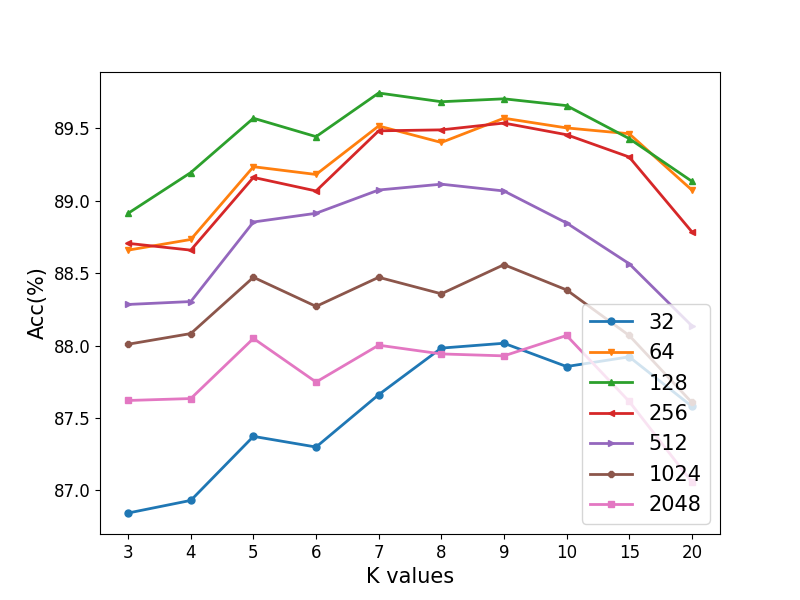
\includegraphics[width=0.6\linewidth]{img/MLKR_res.png}
        \caption{The Result of MLKR}
        \label{fig:mlkr_res}
    \end{figure}


\subsection{Weakly Supervised Metric Learning}

\subsubsection{ITML: Information Theoretic Metric Learning}

It is impossible to sample too many number of samples because the  memory for computation is limited.  So the method requires an additional parameter \texttt{num\_constraints}, which indicates that the method will try to build \texttt{num\_constraints} positive pairs and \texttt{num\_constraints} negative pairs. We take different \texttt{num\_constraints} and try to perform classification on the same train-test split of data-set with respect to different $K$ neighbors, to see how the model performs under different scale of pair sampling. The result of experiments on ITML is demonstrated in Table \ref{tab:itml}.

\begin{table}[h]
\centering
\caption{KNN Accuracy of ITML with different sample numbers \label{tab:itml}}
\begin{tabular}{cccccc}
\hline
K   & 50       & 100      & 200      & 500      & 1000     \\ \hline
3   & 88.177\% & 87.367\% & 86.208\% & \textbf{82.812}\% & \textbf{79.597}\% \\
4   & 88.043\% & 86.871\% & 85.887\% & 82.202\% & 79.168\% \\
5   & 88.599\% & \textbf{87.601}\% & \textbf{86.322}\% & 82.618\% & 79.463\% \\
6   & 88.573\% & 87.159\% & 86.034\% & 82.142\% & 79.074\% \\
7   & \textbf{88.640}\% & 87.367\% & 86.154\% & 82.196\% & 78.900\% \\
8   & 88.506\% & 87.240\% & 85.887\% & 82.042\% & 78.545\% \\
9   & 88.566\% & 87.340\% & 85.967\% & 82.042\% & 78.525\% \\
10  & 88.291\% & 87.119\% & 85.592\% & 81.747\% & 78.163\% \\
15  & 87.809\% & 86.911\% & 85.478\% & 80.883\% & 77.507\% \\
20  & 87.487\% & 86.376\% & 85.036\% & 80.293\% & 76.790\% \\
30  & 86.838\% & 85.451\% & 84.199\% & 79.081\% & 75.484\% \\ \hline
Avg & \textbf{88.139\%} & 86.982\% & 85.706\% & 81.642\% & 78.292\% \\ \hline
\end{tabular}
\end{table}

It can be seen that fewer samples and a relatively small K leads to better performance on ITML metric.

Note that 50 samples are only a very small fraction of the whole data-set, and that larger sample numbers result in a cascade in the classification accuracy, indicating that the metrics we learned from ITML will not help improve the classification performance. We wonder if there exists an improved metric learning solution based on ITML. It turned out that preprocessing the data-set with \emph{PCA} can help ITML exert its true power.

We perform PCA on the original data-set and reduce every data point from 2048 dimensions to 64 dimensions. The KNN accuracy with ITML learned metrics is listed in Table \ref{tab:itml2}.

\begin{table}[h]
\centering
\caption{KNN Accuracy on PCA reduced data-set of ITML with different sample numbers \label{tab:itml2}}
\footnotesize
\begin{tabular}{ccccccccc}
\hline
K   & 50       & 100      & 200      & 500      & 1000     & 5000     & 10000    & 20000    \\ \hline
3   & 87.360\% & 87.528\% & 88.465\% & 88.887\% & 89.276\% & 89.175\% & 89.229\% & 89.249\% \\
4   & 87.220\% & 87.561\% & 88.445\% & 89.008\% & 89.162\% & 89.236\% & 89.323\% & 89.524\% \\
5   & 87.682\% & 87.943\% & 89.041\% & 89.624\% & 89.805\% & 89.778\% & 89.912\% & 89.865\% \\
6   & 87.688\% & 88.090\% & 89.102\% & 89.624\% & 89.685\% & 89.718\% & 89.651\% & 90.107\% \\
7   & 87.943\% & \textbf{88.305\%} & \textbf{89.457\%} & 89.510\% & \textbf{89.872\%} & 89.939\% & \textbf{90.113\%} & 90.073\% \\
8   & 87.923\% & 88.204\% & 89.129\% & 89.571\% & 89.798\% & 89.993\% & 89.966\% & \textbf{90.274\%} \\
9   & \textbf{87.990\%} & 88.110\% & 89.296\% & 89.751\% & 89.785\% & 90.013\% & 90.086\% & 90.261\% \\
10  & 87.909\% & 88.177\% & 89.269\% & \textbf{89.812\%} & 89.678\% & \textbf{90.127\%} & 90.073\% & 90.173\% \\
15  & 87.595\% & 87.856\% & 89.055\% & 89.772\% & 89.772\% & 90.026\% & 90.033\% & 90.167\% \\
20  & 87.534\% & 87.494\% & 88.928\% & 89.597\% & 89.577\% & 89.952\% & 89.973\% & 90.026\% \\
30  & 87.012\% & 86.885\% & 88.305\% & 89.209\% & 89.082\% & 89.584\% & 89.651\% & 89.671\% \\ \hline
Avg & 87.623\% & 87.832\% & 88.954\% & 89.488\% & 89.590\% & 89.776\% & 89.819\% & \textbf{89.945}\% \\ \hline
\end{tabular}
\end{table}

After PCA, The training accuracy grows monotonously as we increase the sampling number, indicating that the ITML metric learning distance can indeed boost the classification performance. We conclude that the accuracy of ITML metrics on PCA-reduced data-set can outperform the euclidean metrics with sufficient sampling.

\begin{figure}
    \centering
    \begin{minipage}[t]{0.48\linewidth}
        \centering
        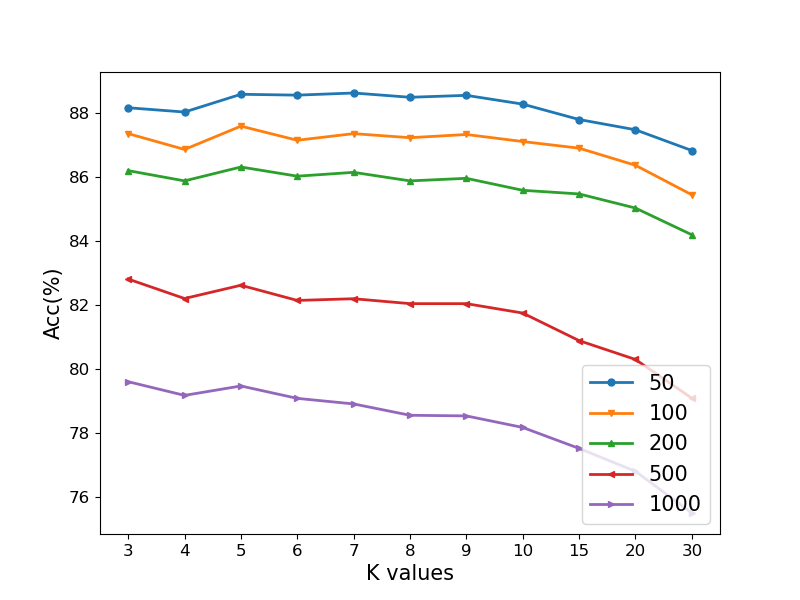
\includegraphics[width=1.0\linewidth]{img/ITML-k.png}
        \caption{Accuracy of ITML metric learning}
        \label{fig:itml}
    \end{minipage}
    \begin{minipage}[t]{0.48\linewidth}
        \centering
        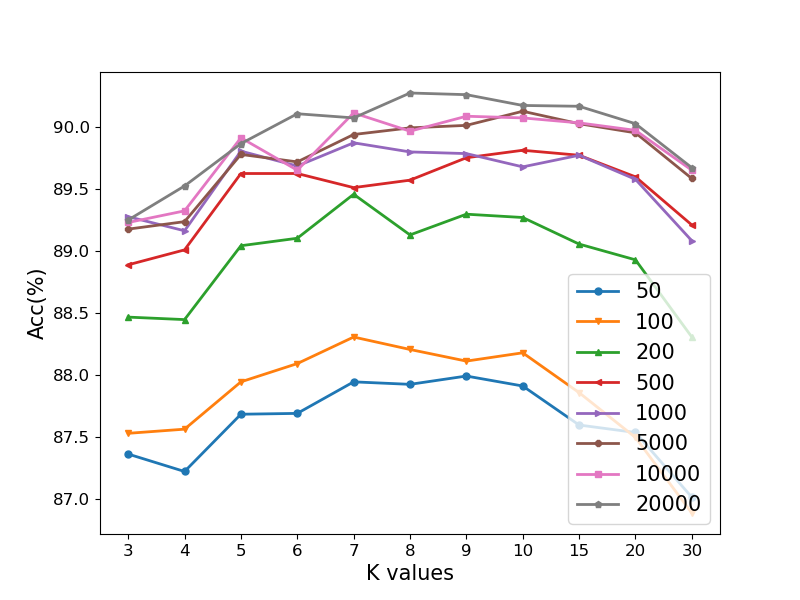
\includegraphics[width=1.0\linewidth]{img/ITML-PCA-k.png}
        \caption{Accuracy of ITML after PCA}
        \label{fig:itml-pca}
    \end{minipage}
\end{figure}


\subsubsection{LSML: Least Squared-residual Metric Learning}

We take different \texttt{num\_constraints} and try to perform classification on the same train-test split of data-set with respect to different $K$ neighbors. The result of experiments on LSML is demonstrated in Table \ref{tab:lsml}.

\begin{table}[h]
\centering
\caption{KNN Accuracy of LSML with different sample numbers \label{tab:lsml}}
\begin{tabular}{cccccc}
\hline
K   & 50       & 100      & 200      & 500      & 1000     \\ \hline
3   & 88.834\% & 88.894\% & 88.834\% & 89.062\% & 89.088\% \\
4   & 88.921\% & 88.834\% & 88.995\% & 89.149\% & 89.169\% \\
5   & 89.289\% & 89.242\% & 89.370\% & 89.544\% & 89.396\% \\
6   & 89.229\% & 89.242\% & 89.396\% & 89.484\% & 89.396\% \\
7   & \textbf{89.390\%} & \textbf{89.430\%} & \textbf{89.423\%} & \textbf{89.591\%} & \textbf{89.524\%} \\
8   & 89.236\% & 89.155\% & 89.196\% & 89.410\% & 89.350\% \\
9   & 89.303\% & 89.329\% & 89.296\% & 89.463\% & 89.490\% \\
10  & 89.196\% & 89.068\% & 89.175\% & 89.423\% & 89.269\% \\
15  & 88.961\% & 88.961\% & 89.008\% & 89.075\% & 88.901\% \\
20  & 88.686\% & 88.619\% & 88.546\% & 88.767\% & 88.539\% \\
30  & 87.923\% & 87.970\% & 87.775\% & 88.050\% & 87.722\% \\ \hline
Avg & 88.997\% & 88.977\% & 89.001\% & \textbf{89.183}\% & 89.077\% \\ \hline
\end{tabular}
\end{table}

It can be seen that the number of samples makes minor difference to the classification accuracy and that a moderate K is preferred for LSML metric learning.

\begin{table}[h]
\centering
\caption{KNN Accuracy of LSML on PCA-reduced data-set with different sample numbers \label{tab:lsml2}}
\begin{tabular}{cccccccc}
\hline
    & 200      & 500      & 1000     & 2000     & 5000     & 10000    & 20000    \\ \hline
3   & 89.289\% & 89.544\% & 89.356\% & 89.396\% & 89.417\% & 89.403\% & 89.490\% \\
4   & 89.504\% & 89.551\% & 89.631\% & 89.551\% & 89.624\% & 89.832\% & 89.711\% \\
5   & 90.086\% & 90.247\% & 90.180\% & 90.220\% & 90.214\% & 90.381\% & 90.254\% \\
6   & 90.274\% & 90.435\% & 90.113\% & 90.180\% & 90.274\% & 90.321\% & 90.220\% \\
7   & 90.321\% & 90.529\% & \textbf{90.529\%} & \textbf{90.575\%} & \textbf{90.535\%} & \textbf{90.649\%} & \textbf{90.609\%} \\
8   & \textbf{90.381\%} & 90.274\% & 90.368\% & 90.341\% & 90.374\% & 90.515\% & 90.448\% \\
9   & 90.368\% & \textbf{90.535\%} & 90.475\% & 90.441\% & 90.455\% & 90.616\% & 90.589\% \\
10  & 90.207\% & 90.354\% & 90.348\% & 90.254\% & 90.401\% & 90.495\% & 90.374\% \\
15  & 90.046\% & 90.073\% & 90.261\% & 90.093\% & 90.133\% & 90.254\% & 90.227\% \\
20  & 89.879\% & 89.946\% & 90.013\% & 89.946\% & 90.080\% & 89.999\% & 90.040\% \\
30  & 89.216\% & 89.484\% & 89.484\% & 89.403\% & 89.504\% & 89.584\% & 89.591\% \\ \hline
Avg & 89.961\% & 90.088\% & 90.069\% & 90.036\% & 90.092\% & \textbf{90.186\%} & 90.141\% \\ \hline
\end{tabular}
\end{table}


\begin{figure}
    \centering
    \begin{minipage}[t]{0.48\linewidth}
        \centering
        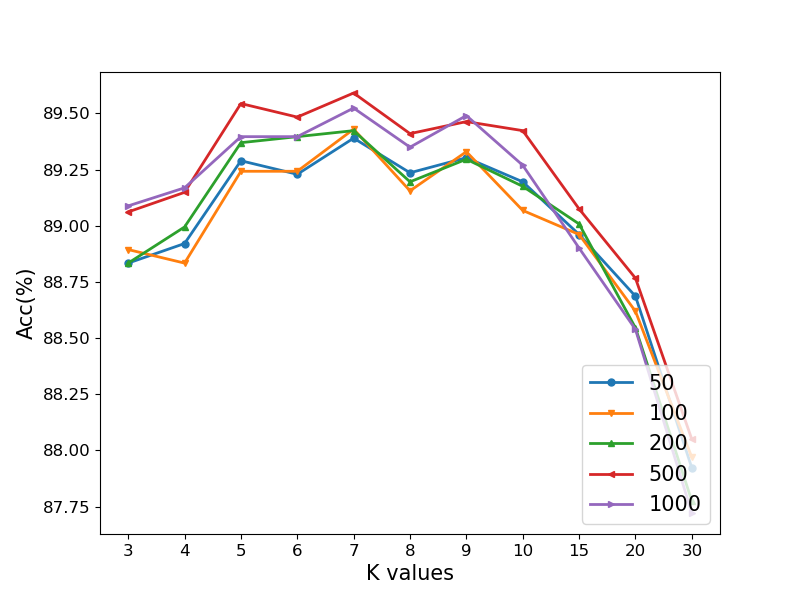
\includegraphics[width=1.0\linewidth]{img/LSML.png}
        \caption{Accuracy of LSML metric learning}
        \label{fig:lsml}
    \end{minipage}
    \begin{minipage}[t]{0.48\linewidth}
        \centering
        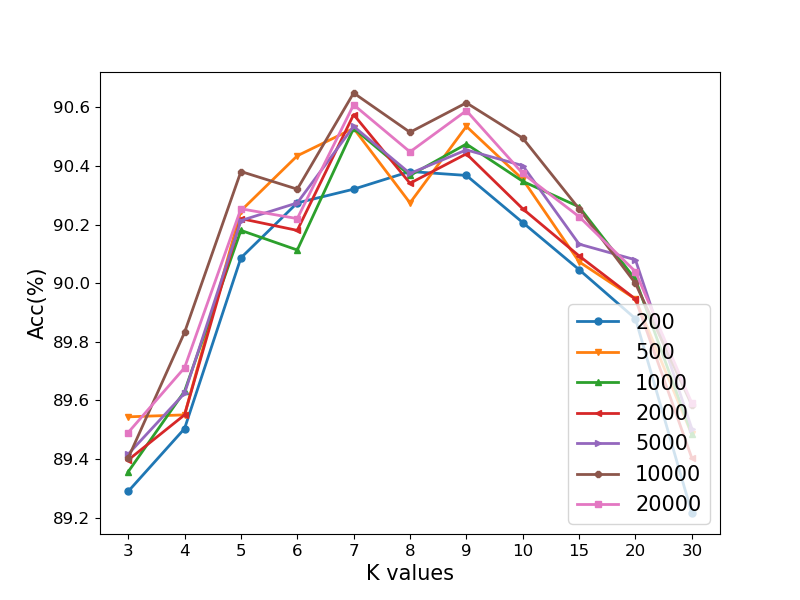
\includegraphics[width=1.0\linewidth]{img/LSML-PCA.png}
        \caption{Accuracy of LSML after PCA}
        \label{fig:lsml-pca}
    \end{minipage}
\end{figure}



Inspired by the experiment results for ITML, we continue to try applying LSML to PCA-reduced dataset. The result is listed in Table \ref{tab:lsml2}. 

Although the improvement after dimensionality reduction is not very significant in accuracy, we may still conclude that PCA is a useful pre-processing technique for weakly supervised metric learning because it enables us to sample more data-points, thus gaining better learned metrics for the KNN classification task. Therefore, for later experiments, we will train the learned metrics after performing PCA on the original data-set.


\subsubsection{SCML: Sparse Compositional Metric Learning}

We first reduce the dimension of the original data-set to 64-dimensions. Then we use SCML to learn the metric and evaluate the KNN classification accuracy. The triplets are sampled by taking 3 neighbours of the same class and 10 neighbours from different classes for each point and then runs the SCML algorithm on these triplets.

The experiment result is shown in Table \ref{tab:scml}. It can be found that SCML does not reach an outstanding performance on our data-set even after PCA.

\begin{table}[h]
\centering
\caption{KNN Accuracy of SCML on PCA-reduced data-set \label{tab:scml}}
\begin{tabular}{cc}
\hline
K   & Accuracy \\ \hline
3   & 86.295\% \\
4   & 86.643\% \\
5   & 87.327\% \\
6   & 87.494\% \\
7   & 87.849\% \\
8   & 87.675\% \\
9   & 87.796\% \\
10  & 87.782\% \\
15  & \textbf{87.956\%} \\
20  & 87.541\% \\
30  & 87.112\% \\ \hline
Avg & 87.406\% \\ \hline
\end{tabular}
\end{table}


\subsubsection{RCA: Relative Components Analysis}

We explore the effect of RCA metric learning by changing our sampling strategy on the PCA-reduced data-set. The experiment result can be found in Table \ref{tab:rca}. Generally speaking, the larger the sampling size, the better the learned metrics. 

\begin{table}[h]
\centering
\caption{KNN Accuracy of RCA on PCA-reduced data-set with different $\mathtt{num\_chunks}\times\mathtt{chunk\_size}$\label{tab:rca}}
\begin{tabular}{cccccccc}
\hline
K   & 100×2             & 100×8             & 100×32            & 200×32            & 500×32            & 500×40            \\ \hline
3   & 84.667\%          & 89.376\%          & 89.705\%          & 89.678\%          & 89.611\%          & 89.624\%          \\
4   & 85.022\%          & 89.329\%          & 89.685\%          & 89.698\%          & 89.685\%          & 89.658\%          \\
5   & \textbf{85.686\%} & 89.765\%          & 90.247\%          & 90.214\%          & 90.167\%          & 90.281\%          \\
6   & 85.659\%          & 89.778\%          & 90.100\%          & 90.207\%          & 90.194\%          & 90.247\%          \\
7   & 85.719\%          & 90.227\%          & 90.354\%          & 90.395\%          & \textbf{90.395\%} & 90.475\%          \\
8   & 85.692\%          & 90.100\%          & 90.294\%          & 90.281\%          & 90.307\%          & 90.448\%          \\
9   & 85.833\%          & 90.234\%          & 90.240\%          & \textbf{90.515\%} & 90.334\%          & 90.395\%          \\
10  & 85.759\%          & \textbf{90.240\%} & \textbf{90.368\%} & 90.455\%          & 90.314\%          & \textbf{90.488\%} \\
15  & 85.645\%          & 89.939\%          & 90.080\%          & 90.361\%          & 90.301\%          & 90.294\%          \\
20  & 85.284\%          & 89.772\%          & 89.879\%          & 90.187\%          & 90.013\%          & 90.080\%          \\
30  & 84.647\%          & 89.350\%          & 89.524\%          & 89.812\%          & 89.604\%          & 89.658\%          \\ \hline
Avg & 85.419\%          & 89.828\%          & 90.043\%          & \textbf{90.164\%} & 90.084\%          & 90.150\%          \\ \hline
\end{tabular}
\end{table}



\section{Conclusion}
\label{sec:conclusion}


Simple distance metrics are the most commonly used metrics in KNN classification, for their calculations are relatively simple. We show that among three Minkowski distances, Euclidean and Manhattan distances perform well, while Chebyshev distance classifies much worse than them. Cosine distance outperforms three Minkowski distances for a better classification performance and it takes fewer computational resources.


Supervised metric learning methods obviously belongs to supervised learning algorithms.  They need to take training samples with labels as input and learn a distance matrix which will project data samples to a new space.  And they made samples in the same class relatively close while samples in different classes are far away from each other . We take several experiments based on LMNN, NCA, LFDA and MLKR algorithms to process the original data, and then use KNN to classify them.  Our experiments result shows that most of these methods can achieve a good accuracy(over 87\%) if we take appropriate parameters. Among these methods, LFDA has the best performance and the classification accuracy can reach 92\%. For every specific method, the selection of  K and feature dimension will also affect the result a lot. Usually a moderate value for K will get a better result, for it is enough to learn from neighbors and avoid noise samples at the same time. And reducing the sample dimension can significantly improve the classification efficiency, but it may also lead to the loss of accuracy, we need to find a balance in getting a satisfactory result.



Weakly supervised metric learning methods do not require the label information. They learn metrics based on tuples or triplets of similar/dissimilar data points. We combine several weakly supervised metric learning methods, such as ITML, LSML, SCML and RCA, with KNN classification and carry out a lot of experiments. Our experiments show that since weakly supervised metric learning methods usually involve sampling and take less information from the data-set, most methods cannot perform well on the original AwA2 data-set. To address this problem, by using PCA to reduce the data samples into 64-dimensions, we show that most methods can achieve a good performance similar to that of the original Euclidean metric. Furthermore, with more samples, the classification performance shows an increasing trend, indicating that the metric learning method indeed helps. However, there still exists a trade-off between the high computational cost during training and the limited improved effect brought by metric learning.





\bibliography{main}
\bibliographystyle{plain}


%%%%%%%%%%%%%%%%%%%%%%%%%%%%%%%%%%%%%%%%%%%%%%%%%%%%%%%%%%%%


\appendix



\end{document}